\chapter{4.Basic Morphological Operations}
%These are just my lecture notes with a translation and some example images
%You should be able to find all the images I have used in the folder /images

\newcommand{\mim}[1]{
    \underline{#1}
}

\definecolor{dkgreen}{rgb}{0,0.6,0}
\definecolor{gray}{rgb}{0.5,0.5,0.5}
\definecolor{mauve}{rgb}{0.58,0,0.82}

\lstset{frame=tb,
language=Matlab,
aboveskip=10mm,
belowskip=10mm,
showstringspaces=false,
columns=flexible,
basicstyle={\small\ttfamily},
numbers=left,
identifierstyle=\color{black},
numberstyle=\small\color{gray},
keywordstyle=\color{blue},
commentstyle=\color{dkgreen},
stringstyle=\color{mauve},
breaklines=true,
breakatwhitespace=true,
tabsize=3}

B/W Bild:
\begin{center}
    \begin{tikzpicture}
        \draw (0,0) node[left] {$A=$} node[right] {
\includegraphics[scale = 0.2]{images/Bild1.png}};
    \end{tikzpicture}
\end{center}
\mim{Structural element}:
\begin{center}
    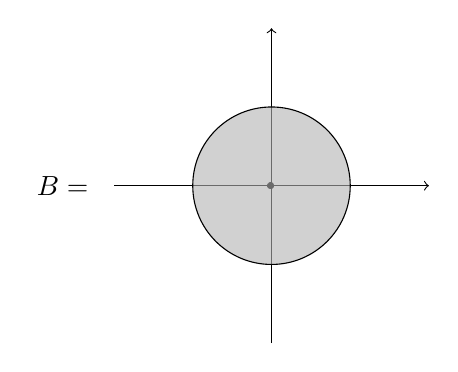
\begin{tikzpicture}[scale = 2]
            \draw[->] (0,-1) -- (0,0) node {\tiny \textbullet} -- (0,1);
            \draw[->] (-1,0) -- (0,0) -- (1,0);
            \fill[black!30, opacity = 0.6] (0,0) circle (0.5);
            \draw (0,0) circle (0.5);
            \draw (-1.1,0) node[left] {$B=$};
    \end{tikzpicture}
\end{center}

\section{Operations on A and B}
\[A+B := \{a + b : a \in A, b \in B\}\]
This is called \underline{dilation}.\\
You might imagine that at every dark point in the image $A$ the Structurelement is applied.
\begin{center}
    \begin{tikzpicture}
        \draw (0,0) node[left] {$A+B=$} node[right] {
\includegraphics[scale = 0.2]{images/Bild1dil.png}};
    \end{tikzpicture}
\end{center}

Image created in Matlab through:
\begin{lstlisting}
I=imread('Bild1.png');
se=strel('disk',40,8);
I2=imcomplement(imdilate(imcomplement(I),se));%I am using the complement of the image here so that the structural element is applied to the dark parts of the image
imshow(I2);
\end{lstlisting}

\[A-B := \{a : a + B \subset A\}\]
This is called \mim{erosion}.\\
You can imagine that you search for the points in which the structural element fits.
\begin{center}
    \begin{tikzpicture}
        \draw (0,0) node[left] {$A-B=$} node[right] {
\includegraphics[scale = 0.2]{images/Bild1erode.png}};
    \end{tikzpicture}
\end{center}

Image created in Matlab thorugh:
\begin{lstlisting}
I=imread('Bild1.png');
se=strel('disk',20,8);
I2=imcomplement(imerode(imcomplement(I),se));
imshow(I2);
\end{lstlisting}

One may quickly realize that $A \neq (A+B)-B$, so a new Operation is introduced:
\[A \bullet B := (A+B)-B\]
This is called \mim{closing} and is used to e.g. remove noise. In the example image you might notice that the upper window is missing.
\begin{center}
    \begin{tikzpicture}
        \draw (0,0) node[left] {$A \bullet B=$} node[right] {
\includegraphics[scale = 0.2]{images/Bild1close.png}};
    \end{tikzpicture}
\end{center}

Image created in Matlab thorugh:
\begin{lstlisting}
I=imread('Bild1.png');
se=strel('disk',20,8);
I2=imcomplement(imdilate(imcomplement(I),se));
I3=imcomplement(imerode(imcomplement(I2),se));
imshow(I3);
\end{lstlisting}

The inverse also exists:
\[ A \circ B := (A-B)+B\]
This is called \mim{opening}.

This time with a new example:

\begin{center}
    \begin{tikzpicture}
        \draw (0,0) node[left] {$A=$} node[right] {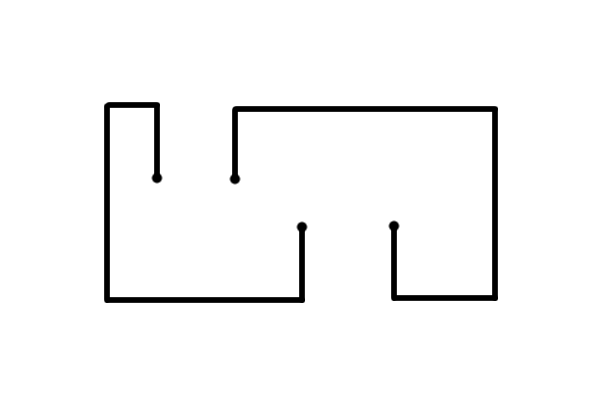
\includegraphics[scale = 0.2]{images/Bild2.png}};
    \end{tikzpicture}
\end{center}

\begin{center}
    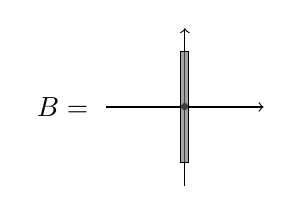
\begin{tikzpicture}
        \draw[->] (0,-1) -- (0,0) node {\tiny \textbullet} -- (0,1);
        \draw[->] (-1,0) -- (0,0) -- (1,0);
        \fill[black!60, opacity = 0.6] (-0.05,-0.7) rectangle (0.05,0.7);
        \draw (-0.05,-0.7) rectangle (0.05,0.7);
        \draw (-1.1,0) node[left] {$B=$};
    \end{tikzpicture}
\end{center}

\begin{center}
    \begin{tikzpicture}
        \draw (0,0) node[left] {$A \circ B =$} node[right] {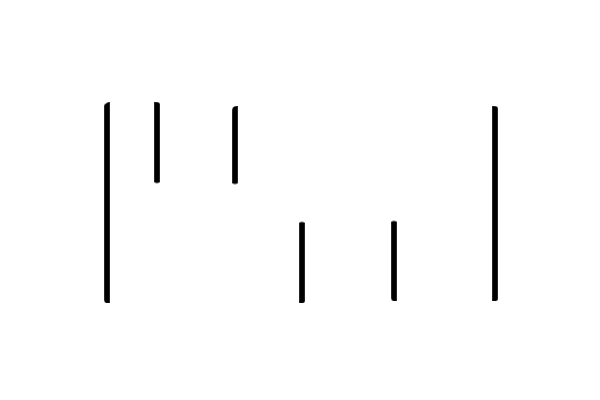
\includegraphics[scale = 0.2]{images/Bild2open.png}};
    \end{tikzpicture}
\end{center}

Image created in Matlab thorugh:
\begin{lstlisting}
I=imread('Bild2.png');
se=strel('line',10,90);
I2=imcomplement(imerode(imcomplement(I),se));
I3=imcomplement(imerode(imcomplement(I2),se));
imshow(I3);
\end{lstlisting}